\begin{figure}[htbp]
\section*{SMAD3}
\centering
\begin{subfigure}[b]{0.95\textwidth}
\centering
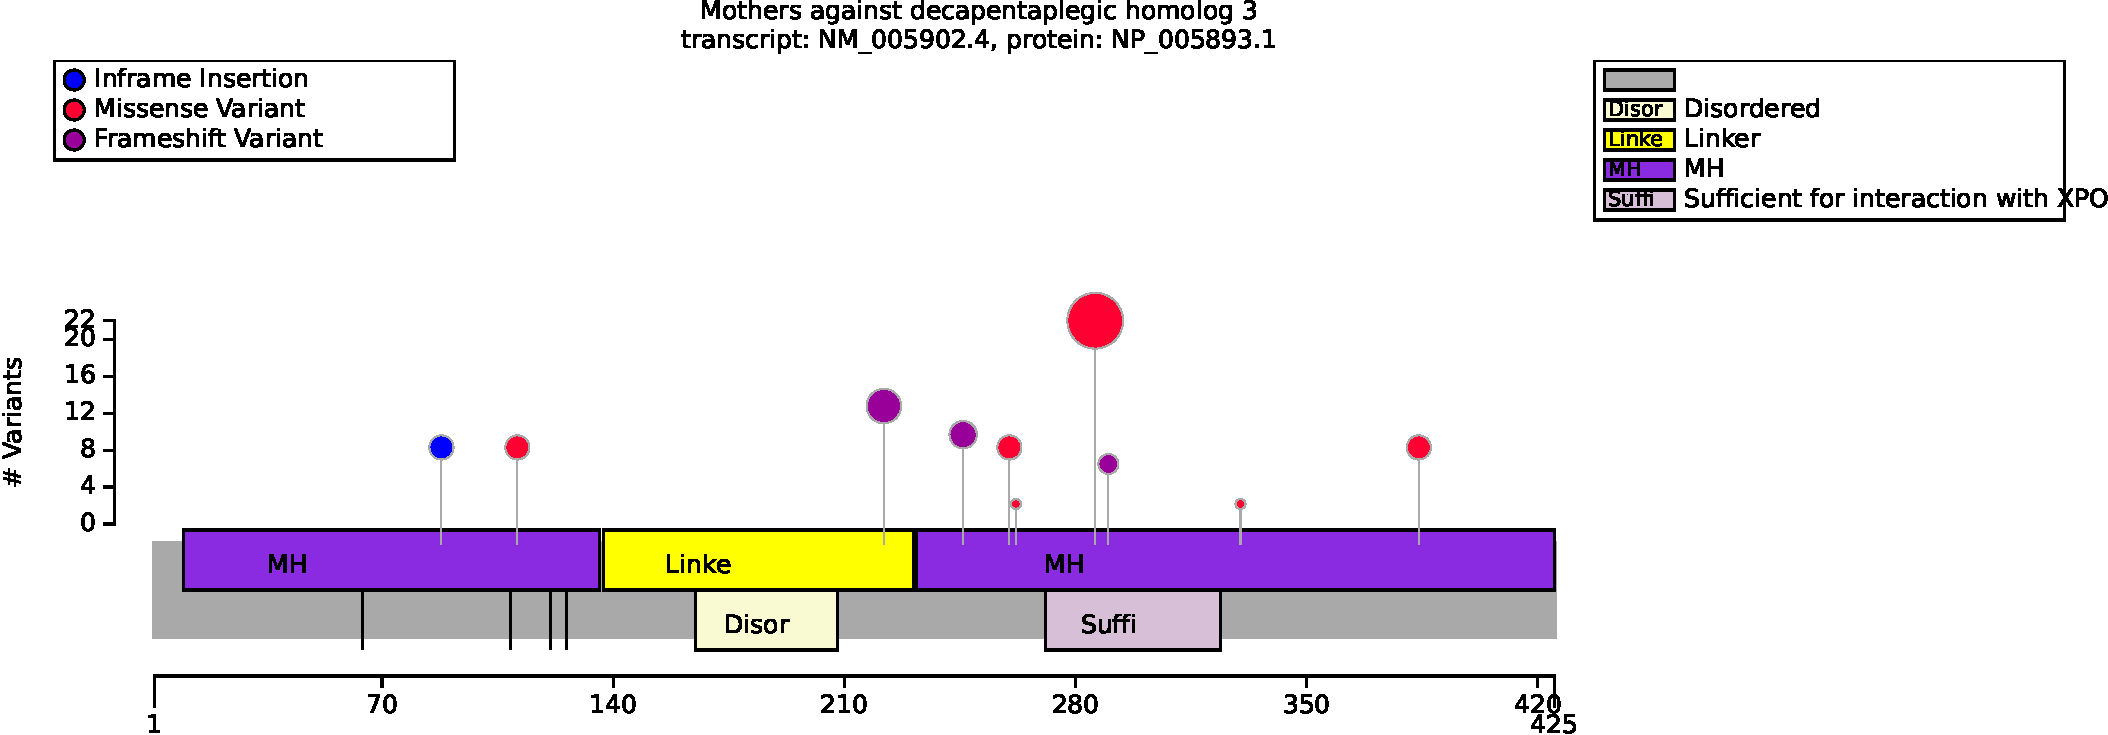
\includegraphics[width=\textwidth]{ img/SMAD3_protein_diagram.pdf} 
\captionsetup{justification=raggedright,singlelinecheck=false}
\caption{Distribution of variants in SMAD3}
\end{subfigure}

\vspace{2em}

\begin{subfigure}[b]{0.95\textwidth}
\centering
\resizebox{\textwidth}{!}{
\begin{tabular}{llllrr}
\toprule
HPO term & p.Arg287Trp & Other & p-value & adj. p-value\\
\midrule
Osteoarthritis [HP:0002758] & 19/19 (100\%) & 7/19 (37\%) & $3.72\times 10^{-5}$ & $8.56\times 10^{-4}$\\
\bottomrule
\end{tabular}
}
\captionsetup{justification=raggedright,singlelinecheck=false}
\caption{Fisher Exact Test performed to compare HPO annotation frequency with respect to p.Arg287Trp and Other. Total of
        23 tests were performed.}
\end{subfigure}
\vspace{2em}
\begin{subfigure}[b]{0.95\textwidth}
\centering
\resizebox{\textwidth}{!}{
\begin{tabular}{llllrr}
\toprule
Genotype (A) & Genotype (B) & total tests performed & significant results\\
\midrule
missense & other & 31 & 0\\
FEMALE & MALE & 31 & 0\\
\bottomrule
\end{tabular}
}
\captionsetup{justification=raggedright,singlelinecheck=false}
\caption{Fisher Exact Test performed to compare HPO annotation frequency with respect to genotypes. }
\end{subfigure}

\vspace{2em}

\caption{ The cohort comprised 49 individuals (22 females, 27 males). 
A total of 30 HPO terms were used to annotate the cohort. Disease diagnosis: Loeys-Dietz syndrome 3 
(OMIM:613795). There was no evidence of a correlation between missense variants and specific 
phenotypic abnormalities. In contrast, there was a statistically significant correlation with 
Arg287Trp and Osteoarthritis. The residue Arg287 is located in the Mad homology 2 (MH2) domain in a 
region that mediates interaction with exportin 4 \cite{PMID_16449645}.
Chesneau et al stated that there is an absence of correlation between the SMAD3 variant type and the occurrence of aortic phenotypes \cite{PMID_32154675}.
To the best of our knowledge an association between Arg287Trp and Osteoarthritis has not been previously noted.
A total of 10 unique variant alleles were found in \textit{SMAD3} (transcript: \texttt{NM\_005902.4}, protein id: \texttt{NP\_005893.1}).}
\end{figure}
